%
% Permission is granted to copy, distribute and/or modify this
% document under the terms of the Creative Common by-nc-sa License
% version 3.0 (CC BY-NC-SA 3.0). A copy of the license can be found at
% http://creativecommons.org/licenses/by-nc-sa/3.0/legalcode.
%

\documentclass[10pt,a4paper]{beamer}
\usepackage[french]{babel}
\usepackage{lmodern}
\usepackage[T1]{fontenc}
\usepackage[utf8]{inputenc}
\usepackage{UBdx}
\usepackage{graphicx}
\usepackage{datetime}
\usepackage[backend=bibtex8]{biblatex}
\usepackage{csquotes}
\addbibresource{biblio.bib}

\newdate{date}{23}{06}{2016}

\newcommand{\highlight}[1]{\textcolor{structure.fg}{\bfseries #1}}
%% \newcommand{\nextsec}{
%%   \begin{frame}<handout:0>
%%     \frametitle{Overview}
%%     \tableofcontents[currentsection]
%%   \end{frame}
%% }oku

\title[Ordonnancement d'application de type stencil]{Ordonnancement d'applications de type stencil sur cluster hybrides CPU/GPU}
\subtitle{}

\author[Lucido Loris]{Lucido Loris\\[-.25em]
  \texttt{\scriptsize <loris.lucido@inria.fr>}}

\institute[Inria Storm]{Stage Optionnel Master (juin - août)\newline LaBRI, Inria Bordeaux Sud-Ouest, Équipe Storm}

\date{\displaydate{date}}

\begin{document}

\begin{frame}
  \vspace{3.5em}
  \titlepage
\end{frame}

%% \begin{frame}
%%   \frametitle{Overview}
%%   \tableofcontents
%% \end{frame}

%%%%%%%%%%%%%%%%%%%%%%%%%%%%%%%%%%%%%%%%%%%

\begin{frame}
  \frametitle{What's a stencil application?}
  \begin{itemize}
%%  expliquer en une phrase pourquoi c'est beaucoup utilisé: discrétisation de
%% phénomènes physiques locaux sur des grilles régulières
  \item Class of algorithms mainly used in simulation
  \item Example : Fluid dynamics
  \item We update one cell based on the content of her neighborhood
  \end{itemize}
  \begin{figure}
    \center
    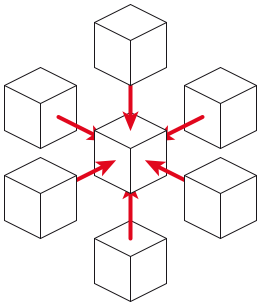
\includegraphics[width=0.25\linewidth]{figures/3D_stencil.png} \\
    \small{6-point 3D stencil~\cite{6pstencil}.}
  \end{figure}
\end{frame}

\begin{frame}
  \frametitle{Abelian sandpiles}
  %% \begin{itemize}
  %% \end{itemize}
  \begin{figure}
    \center
    \includegraphics[width=1\linewidth]{figures/sandpile.png} \\
    \small{Abelian sandpile with max height 4~\cite{sandpile}.}
  \end{figure}
\end{frame}

\begin{frame}
\frametitle{Stencil computation scheme}
  \begin{itemize}
  \item A lot of communication with neighborhood
  \item \textit{Memory bound :} ratio memory access per computation is high
  \item We can't always overlap data transfers between nodes with computation
  \end{itemize}
\end{frame}

\begin{frame}
\frametitle{Save bandwidth between all memory nodes}
  \begin{itemize}
    \vfill
  \item Work on data locality:
    \begin{itemize}
    \item Space locality
    \item Temporal locality
    \end{itemize}
    \vfill
  \item Two schedulers take into account data locality in StarPU for now: \texttt{ws} and \texttt{lws} (\textit{work stealing})
    \vfill
  \end{itemize}
\end{frame}

\begin{frame}
  \frametitle{Work stealing scheduling}
  \vfill
  \begin{figure}
    \center
    \includegraphics[width=0.5\linewidth]{figures/sched_ws.pdf} \\
    \small{Work stealing scheduling.}
  \end{figure}
  \vfill
\end{frame}

\begin{frame}
\frametitle{Off-line Feedback}
\begin{itemize}
\item Parsing FxT traces :
\end{itemize}
\begin{figure}
  \center
  \includegraphics[width=1\linewidth]{figures/locality_attila_ws.png} \\
  \small{Trace generated during Simgrid execution.} \\
  \vfill
  \includegraphics[width=0.3\linewidth]{figures/xpm_legend.pdf}
  \end{figure}
%% un peu comme les diagrammes de gantt observable avec vite
\end{frame}

\begin{frame}
\frametitle{Off-line Feedback}
\begin{figure}
  \center
  \includegraphics[width=0.6\linewidth]{figures/locality_attila_ws_zoom.png} \\
  \vfill
  \includegraphics[width=0.3\linewidth]{figures/xpm_legend.pdf}
\end{figure}
\end{frame}

\begin{frame}
  \frametitle{References}
\printbibliography
\end{frame}

\begin{frame}
  \Huge{\centerline{Thanks for your attention!}}
\end{frame}

\begin{frame}
  \frametitle{Annexes}
\end{frame}

\begin{frame}
  \frametitle{Work stealing scheduling}
  \begin{itemize}
  \vfill
    %% ws vole d'abord aux voisins: les cpus qui partagent le même cache L2, puis L3,
    %% puis sur le même nœud NUMA, etc
  \item Flags \texttt{USE\_LOCALITY} and \texttt{USE\_LOCALITY\_TASKS} (both experimental)
    \vfill
    %% modifications in applications
  \item Add \texttt{STARPU\_LOCALITY} mode to a buffer in a StarPU codelet
  \vfill
  \end{itemize}
\end{frame}

\end{document}
